% Copyright 2004 by Till Tantau <tantau@users.sourceforge.net>.
%
% In principle, this file can be redistributed and/or modified under
% the terms of the GNU Public License, version 2.
%
% However, this file is supposed to be a template to be modified
% for your own needs. For this reason, if you use this file as a
% template and not specifically distribute it as part of a another
% package/program, I grant the extra permission to freely copy and
% modify this file as you see fit and even to delete this copyright
% notice. 

\documentclass{beamer}
\usepackage{multirow}
\usepackage{subfig}
\usepackage{subfloat}
\usepackage{color}
\usepackage{graphicx}
\usepackage{tikz}
% Optional PGF libraries
\usepackage{pgflibraryarrows}
\usepackage{pgflibrarysnakes}

% There are many different themes available for Beamer. A comprehensive
% list with examples is given here:
% http://deic.uab.es/~iblanes/beamer_gallery/index_by_theme.html
% You can uncomment the themes below if you would like to use a different
% one:
%\usetheme{AnnArbor}
%\usetheme{Antibes}
%\usetheme{Bergen}
%\usetheme{Berkeley}
%\usetheme{Berlin}
%\usetheme{Boadilla}
%\usetheme{boxes}
%\usetheme{CambridgeUS}
%\usetheme{Copenhagen}
%\usetheme{Darmstadt}
%\usetheme{default}
%\usetheme{Frankfurt}
%\usetheme{Goettingen}
%\usetheme{Hannover}
%\usetheme{Ilmenau}
%\usetheme{JuanLesPins}
%\usetheme{Luebeck}
\usetheme{Madrid}
%\usetheme{Malmoe}
%\usetheme{Marburg}
%\usetheme{Montpellier}
%\usetheme{PaloAlto}
%\usetheme{Pittsburgh}
%\usetheme{Rochester}
%\usetheme{Singapore}
%\usetheme{Szeged}
%\usetheme{Warsaw}

\title{Solving Elastic Wave Equation in 3D by SBP4 with Curvilinear domain and Mesh Refinement}

\author[Lu Zhang]{Lu Zhang\\
Mentor: Anders Petersson }

\institute[LLNL] % (optional, but mostly needed)
{
  CASC Division\\
  Lawrence Livermore National Lab
  }
% - Use the \inst command only if there are several affiliations.
% - Keep it simple, no one is interested in your street address.

\date{Aug. 8, 2019}
% - Either use conference name or its abbreviation.
% - Not really informative to the audience, more for people (including
%   yourself) who are reading the slides online

\subject{Theoretical Computer Science}
% This is only inserted into the PDF information catalog. Can be left
% out. 

% If you have a file called "university-logo-filename.xxx", where xxx
% is a graphic format that can be processed by latex or pdflatex,
% resp., then you can add a logo as follows:

% \pgfdeclareimage[height=0.5cm]{university-logo}{university-logo-filename}
% \logo{\pgfuseimage{university-logo}}

% Delete this, if you do not want the table of contents to pop up at
% the beginning of each subsection:
\AtBeginSubsection[]
{
  \begin{frame}<beamer>{Outline}
    \tableofcontents[currentsection,currentsubsection]
  \end{frame}
}

% Let's get started
\begin{document}

\begin{frame}
  \titlepage
\end{frame}

\begin{frame}{Geometry and space discretization}
 \begin{figure}[h]
\begin{center}
\includegraphics[width=0.5\textwidth]{domain.eps}
 \label{fig:convergence_1d}
\end{center}
\end{figure}
Solve:
\[\rho {\bf u}_{tt} = \mathcal{L} {\bf u} + {\bf F},\]
with
\[\mathcal{L} {\bf u} = \sum_{j=1}^3\partial_1(M_{1j}\partial_j{\bf u}) +\partial_2(M_{2j}\partial_j{\bf u})+\partial_3(M_{3j}\partial_j{\bf u}).\]

\end{frame}


\begin{frame}{Geometry and Space Discretization}
 \begin{figure}[h]
\begin{center}
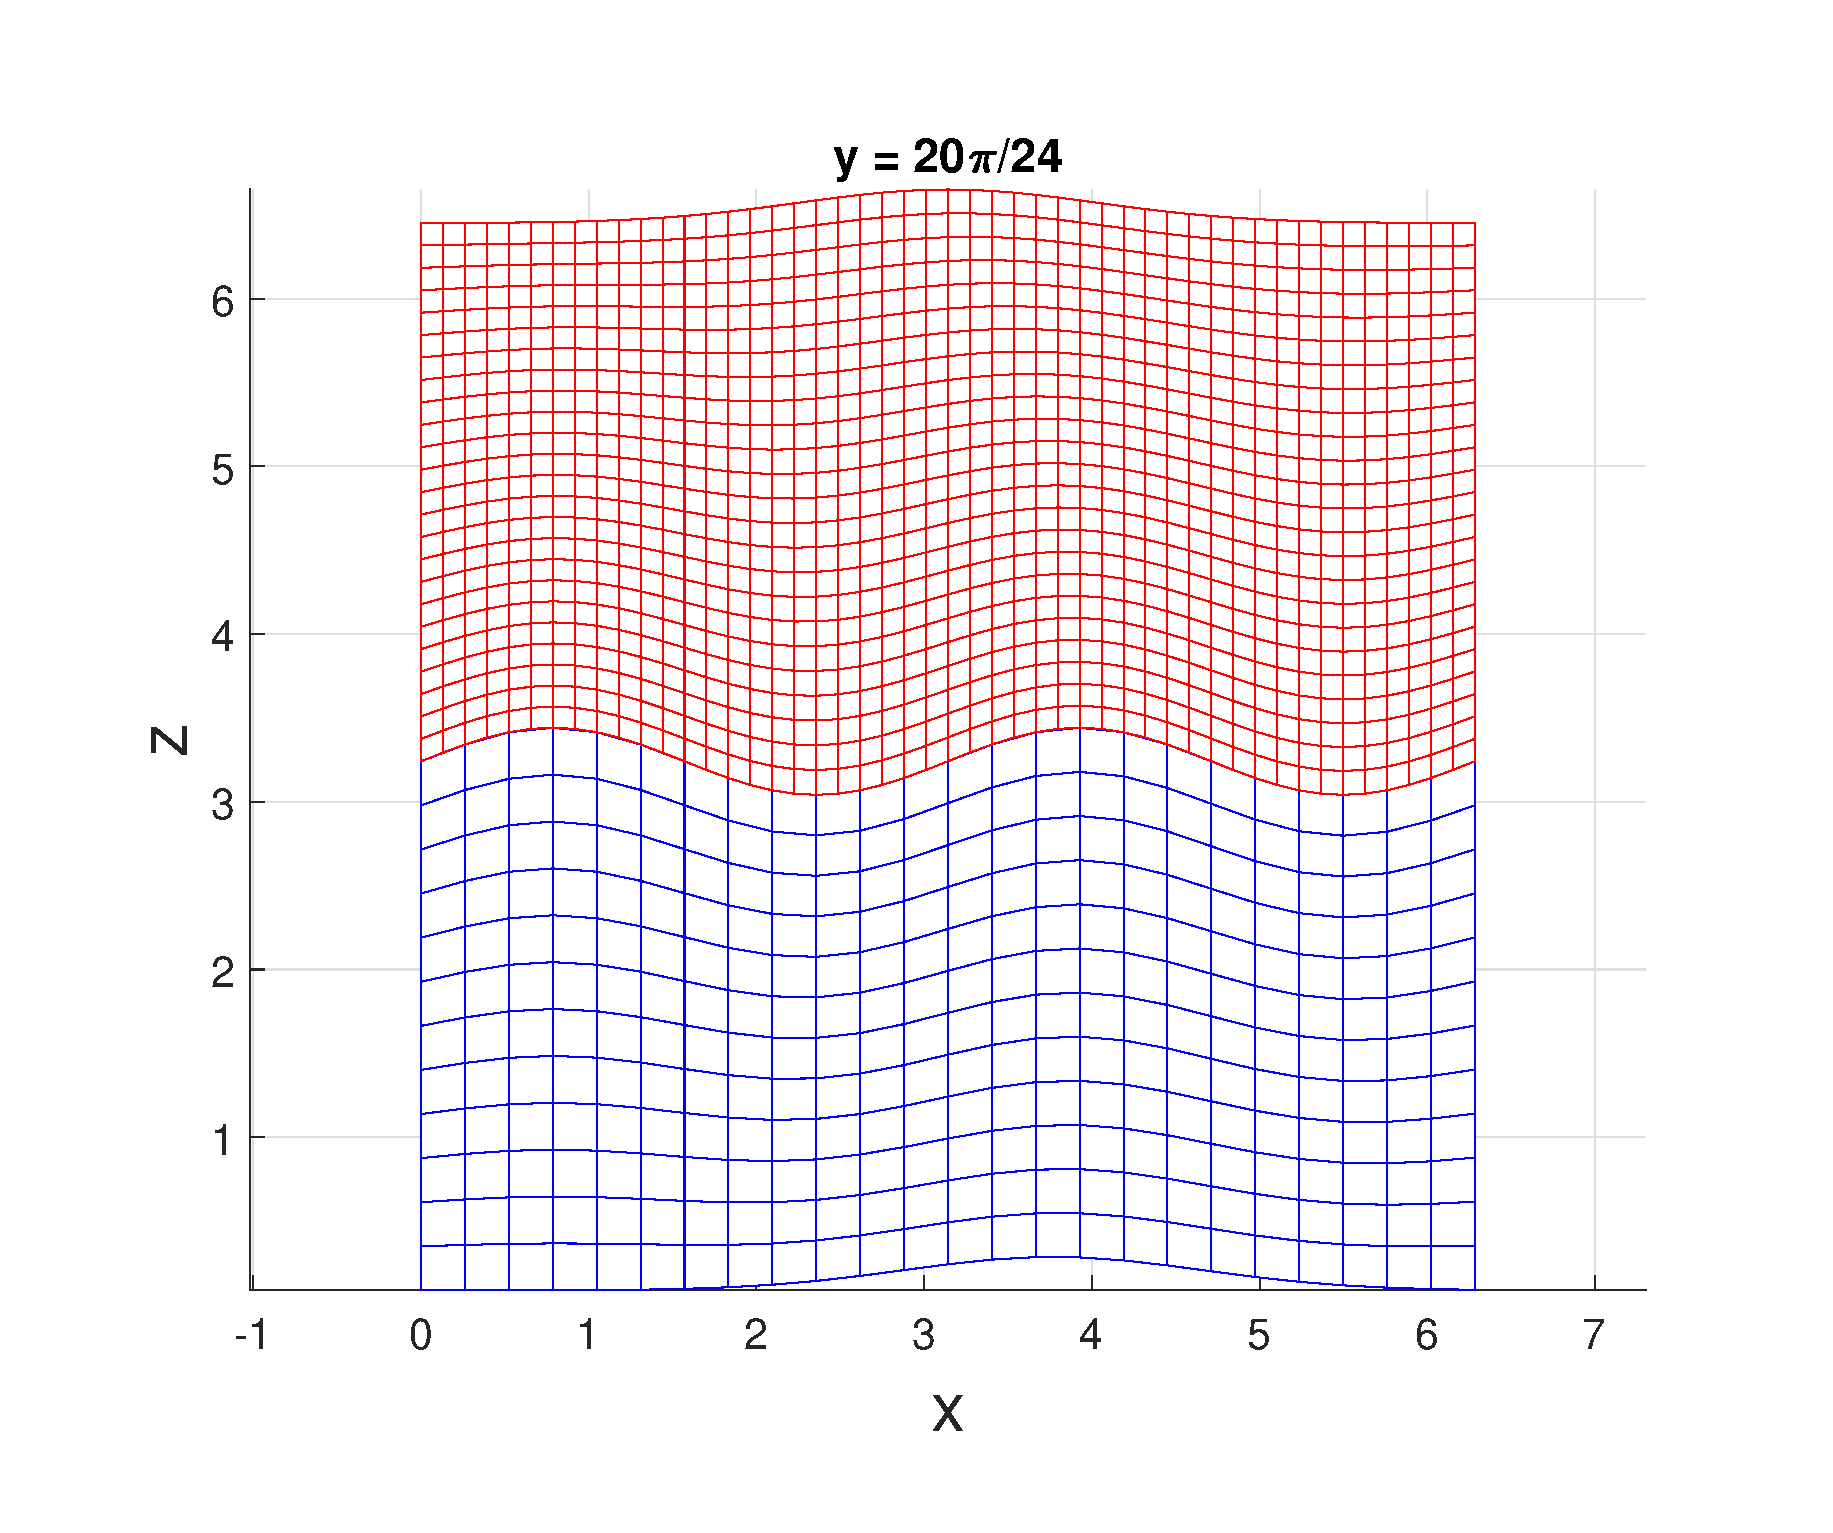
\includegraphics[width=0.33\textwidth]{y11.eps}
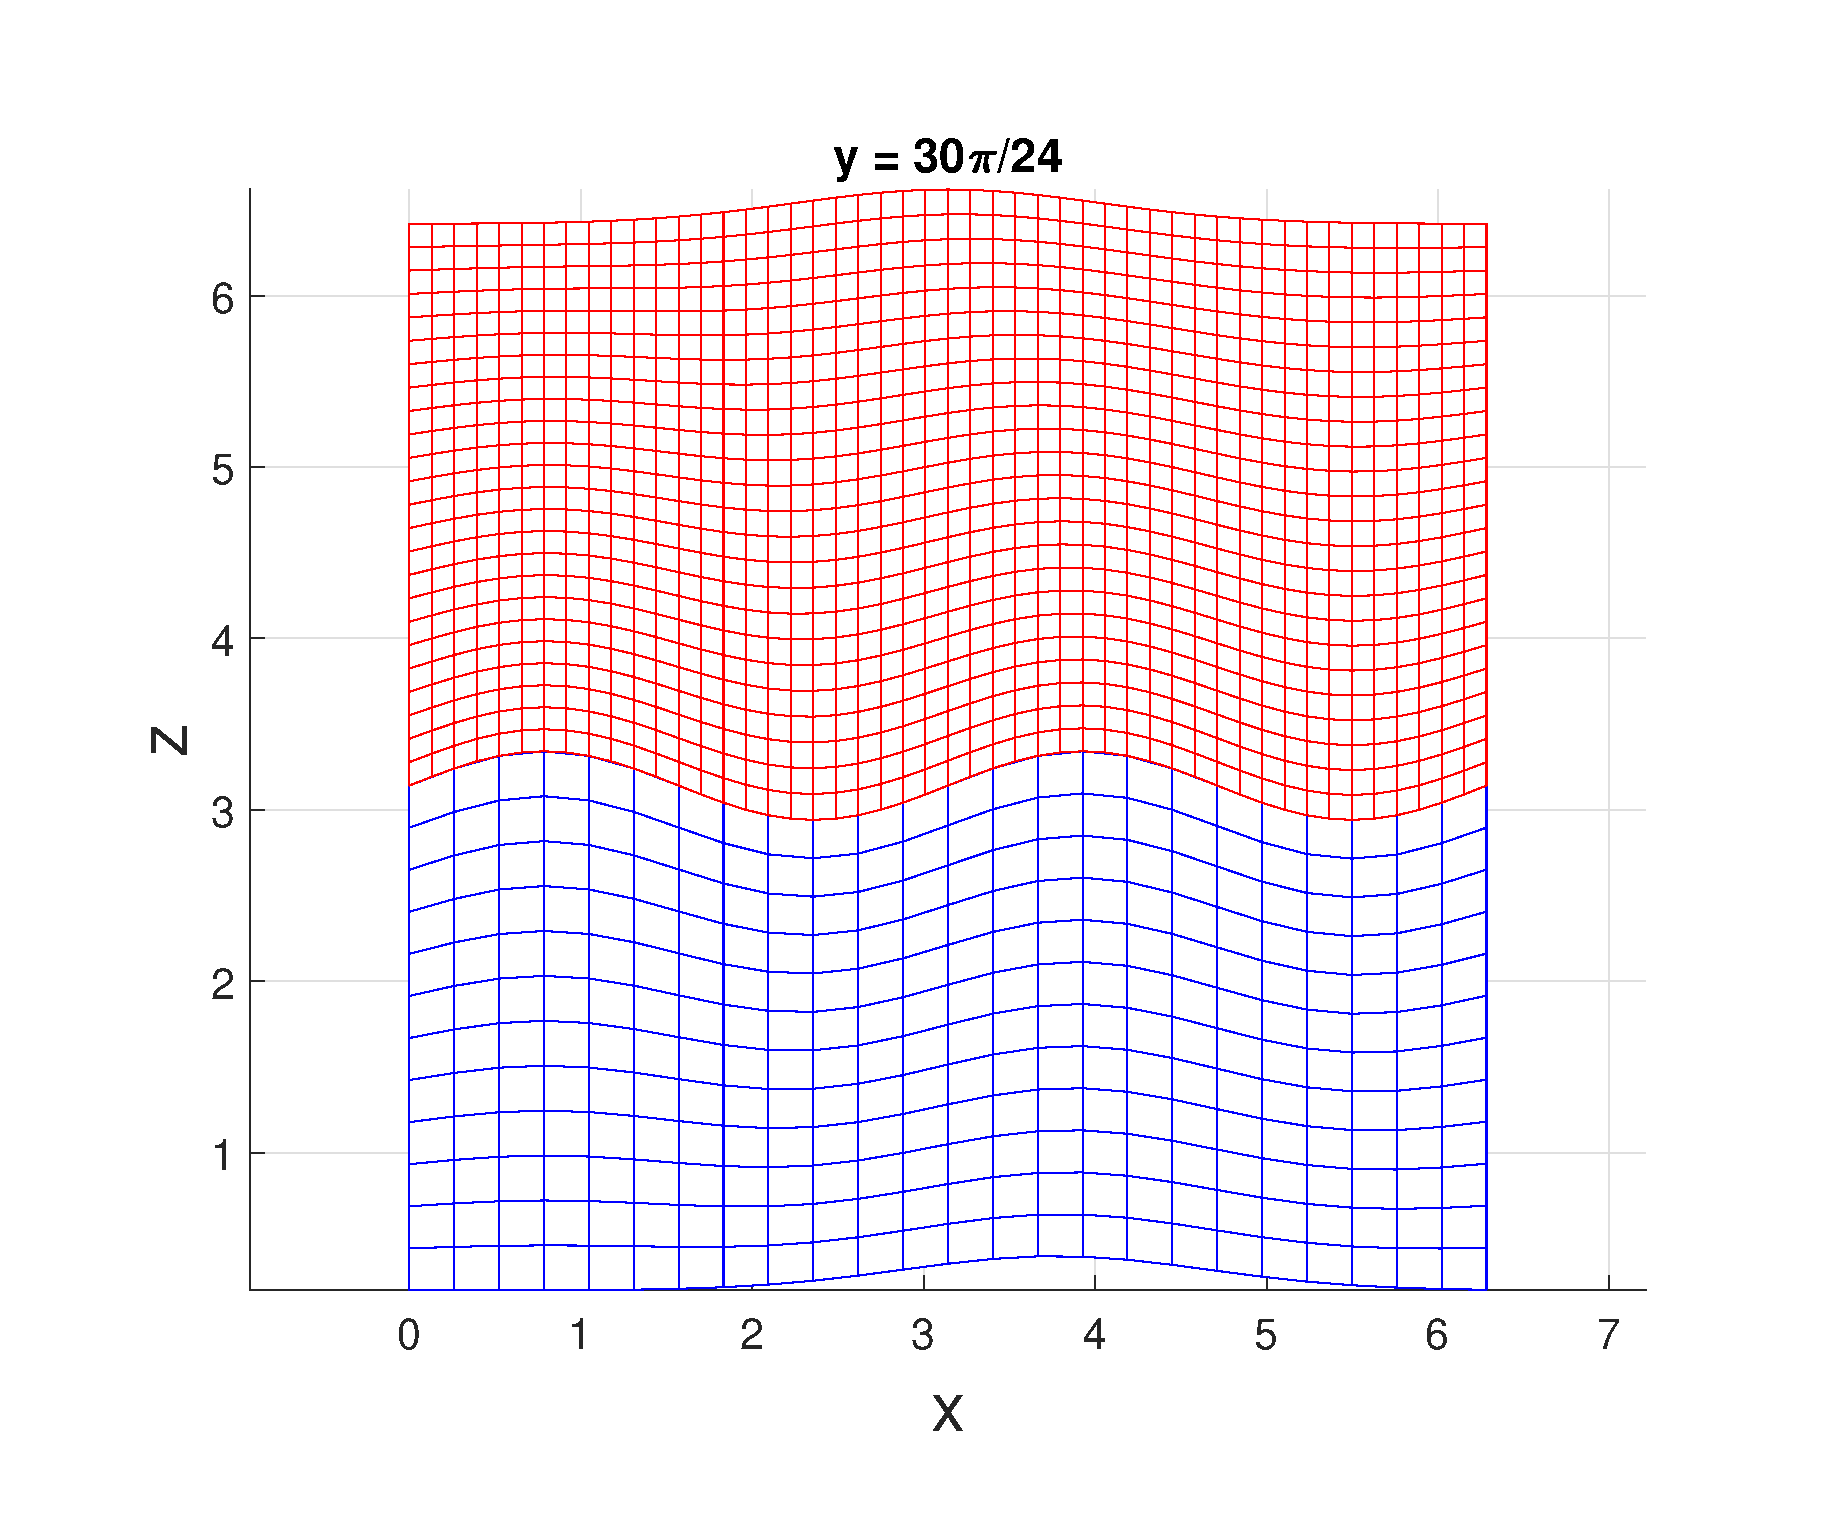
\includegraphics[width=0.33\textwidth]{y16.eps}
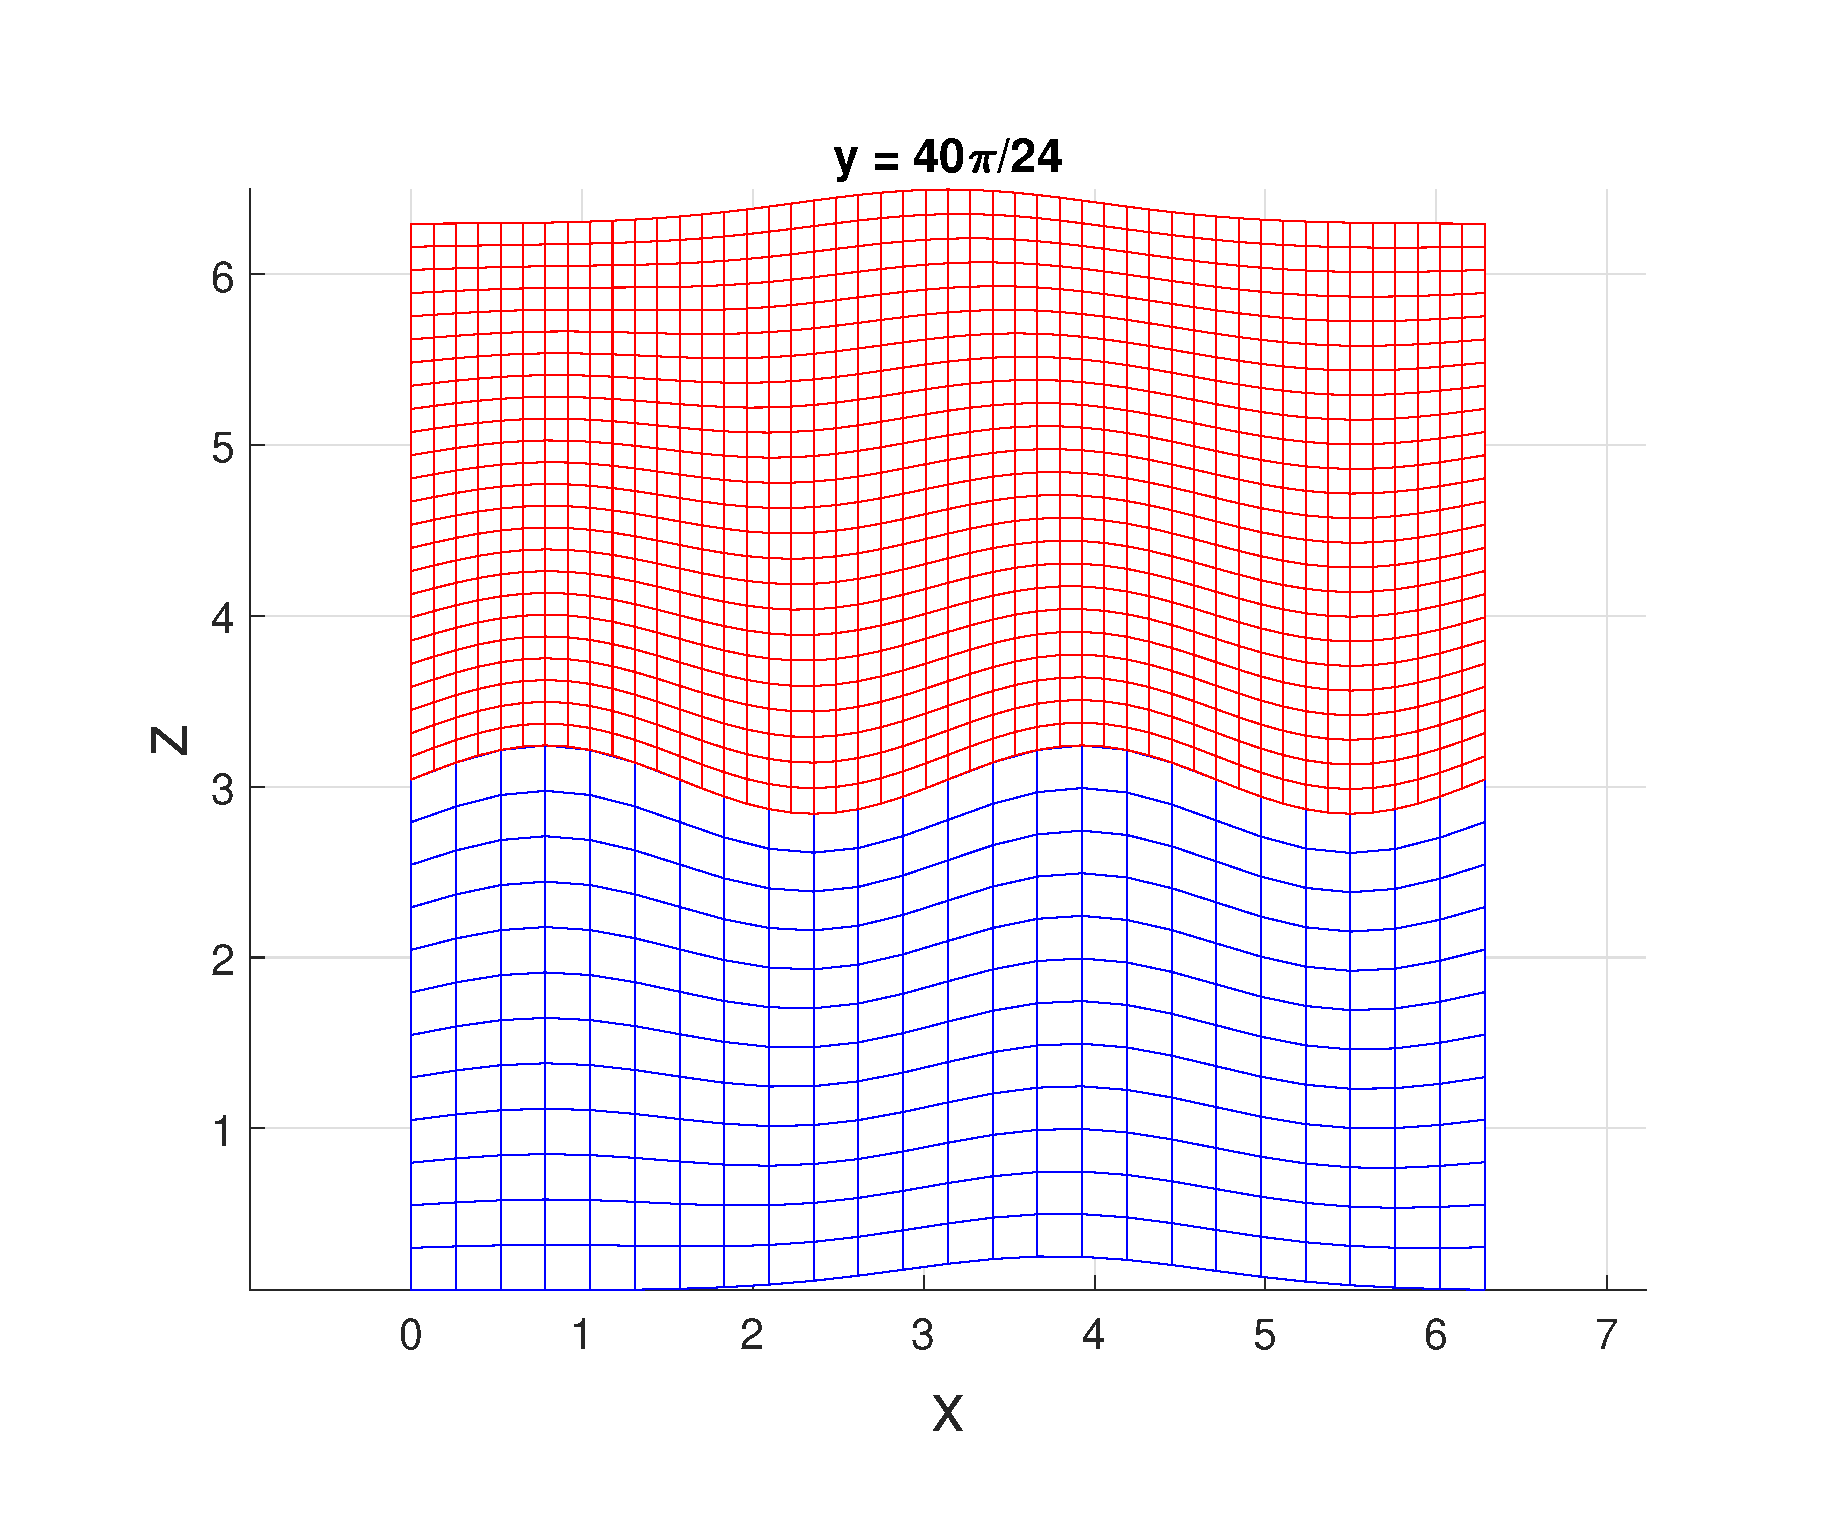
\includegraphics[width=0.33\textwidth]{y21.eps}
\end{center}
\end{figure}  
geometry :
\begin{itemize}
    \item top : $f_t(r_1,r_2)$ 
    \item bottom : $f_b(r_1,r_2)$ 
    \item interface : $f_i(r_1,r_2)$
\end{itemize}
fine domain : $x = r_1L_1, y = r_2L_2, z = r_3f_t(r_1,r_2)+(1-r_3)f_i(r_1,r_2)$\\
coarse domain : $x = r_1L_1, y = r_2L_2, z = r_3f_i(r_1,r_2)+(1-r_3)f_b(r_1,r_2)$

\end{frame}

\begin{frame}{Mesh Refinement Interface}
\begin{figure}[h]
\begin{center}
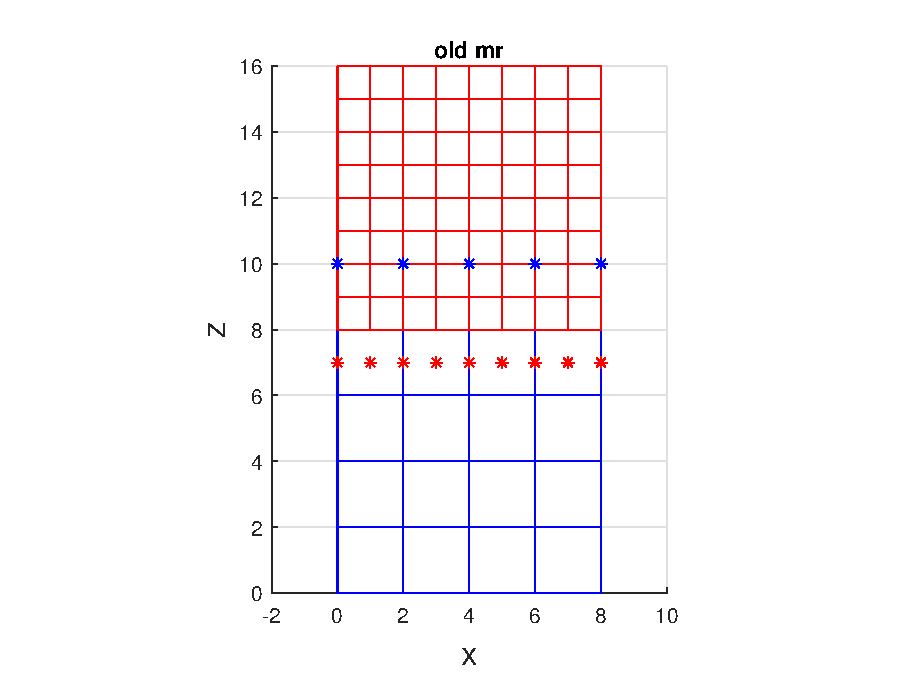
\includegraphics[width=0.35\textwidth]{mrold.eps}
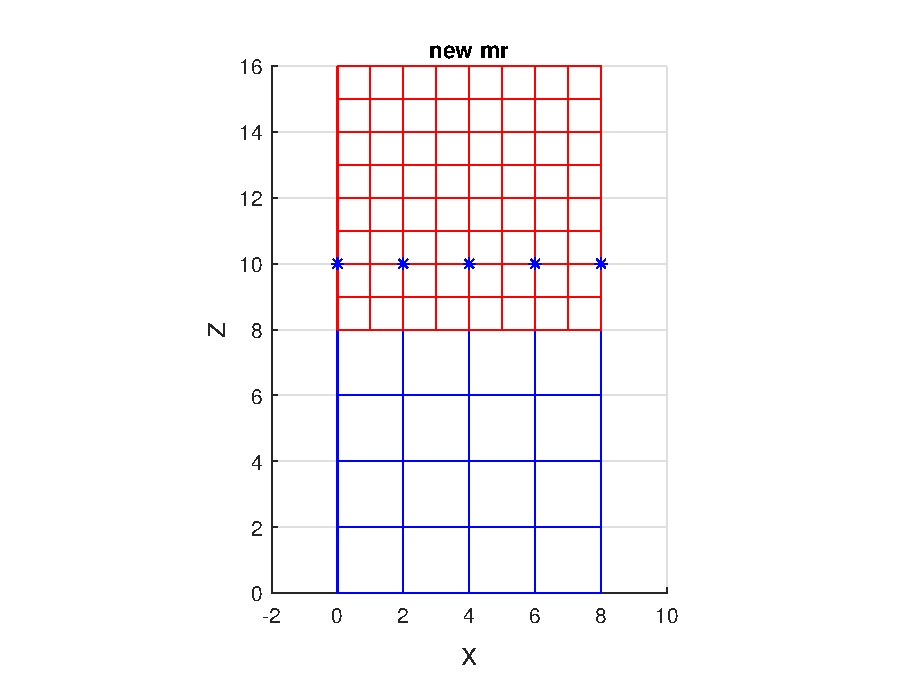
\includegraphics[width=0.35\textwidth]{mrnew.eps}
\end{center}
\end{figure} 
Interface condition:
\begin{itemize}
    \item continuity in displacement: ${\bf u}_f\big|_{\Gamma} = \mathcal{P}({\bf u}_c\big|_{\Gamma})$
    \item continuity in normal stress : 
    \[\sum_{j=1}^3 M_{3j}^c\partial_j {\bf u}_c \big|_{\Gamma} = \mathcal{R}\Big(\sum_{j=1}^3 M_{3j}^f \partial_j {\bf u}_f\big|_{\Gamma}-h_fw_1{\bf \eta}\Big),\]
    with 
    \[{\bf \eta} = \rho_f\big|_{\Gamma}\mathcal{P}\Big((\rho_c)^{-1}\tilde{G}_c(\mu,\lambda)\tilde{u}_c\big|_{\Gamma}\Big)-G_c(\mu,\lambda){\bf u}_f\big|_{\Gamma}\]
\end{itemize}
\end{frame}

\begin{frame}{Errors and Convergence Rate}
material:
\begin{itemize}
    \item $\rho = 2 + \sin(x+0.3)\sin(y+0.3)\sin(z-0.2)$
    \item $\mu = 3 + \sin(3x+0.1)\sin(3y+0.1)\sin(z)$
    \item $\lambda = 21 + \cos(x+0.1)\cos(y+0.1)\sin^2(3z)$
\end{itemize}
~\\
coarse mesh : $2h$; fine mesh : $h$
\begin{table}[htb]
\begin{center}
  \begin{tabular}{|c|c c c|}
  \hline
 2h   & $L_{\infty}^{c}$ & $L_{\infty}^{f}$ & $L^2$  \\
\hline
  $2\pi/24$ &3.9702e-03 ~~~~~~~~ & 3.8742e-03 ~~~~~~~~ & 1.7834e-03 ~~~~~~~~\\
\hline
  $2\pi/48$ &2.6360e-04 (3.91) & 2.6921e-04 (3.85) & 1.0718e-04 (4.06)\\
  \hline 
  $2\pi/96$ &1.8563e-05 (3.83) & 1.6638e-05 (4.02) & 6.3739e-06 (4.07)\\
  \hline
\end{tabular}
\end{center}
\end{table} 

\end{frame}

\begin{frame}{Iterative Solver}
solve : 
\[ Ax = b\]
tol : $1e-7$ 
 \begin{itemize}
     \item Conjugate Gradient method : around $44$ iterations
     \item Preconditioned Conjugate Gradient method : around $9$ iterations
     \item Block Jacobian method : around $13$ iterations
 \end{itemize}  
\end{frame}

\end{document}



